
\chapter{Configurazione Router}

\section{Overview della configurazione}

In questo capitolo andremo a configurare il \it{router 4g} e connetterlo alla VPN.

 % TODO mancano captions

\newsavebox{\myimagea}
\begin{figure}[H]
    \centering%
    \savebox{\myimagea}{
        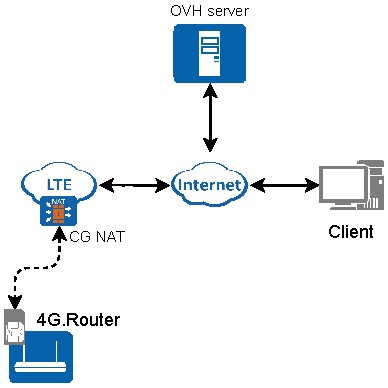
\includegraphics[width=0.45\textwidth]{immagini/diag-router_real}
    }
    \begin{subfigure}{0.4\textwidth}
        \centering
        \usebox{\myimagea}
        \caption{Configurazione iniziale}
        \label{fig:diag-router}
    \end{subfigure}
    \hfill%
    \begin{subfigure}{0.5\textwidth}
        \centering
        \raisebox{\dimexpr.5\ht\myimagea-.5\height\relax}{
            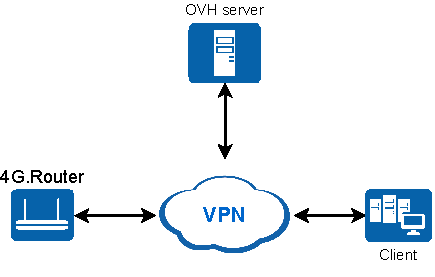
\includegraphics[width=1\linewidth]{immagini/diag-router_goal}
        }
        \caption{Configurazione da raggiungere}
        \label{fig:diag-router1}
    \end{subfigure}
\end{figure}


% <-- section -->
\section{Creazione della configurazione Openvpn}

% TODO da riscrivere
Si devono seguire gli step descritti in sezione \ref{sec:client_keys}, quindi creare la certificate request e firmarla nel \it{server CA}. Per poi usare lo script creato in sezione \ref{sec:script_client} per costruire il file di configurazione:

\begin{bashcode}{Server}{}
$ ./make_config.sh router
\end{bashcode}

Dopodiché si deve spostare il file \code{router.ovpn} dal \it{Server} al \it{Router 4g}, supponiamo di averlo copiato nella cartella \code{/configs}. 

Di default non è presente \it{OpenVPN} nel \it{Router 4g}, lo si può installare con:

\begin{bashcode}{Router 4g}{}
$ opkg update
$ opkg install openvpn
$ opkg install luci-app-openvpn
\end{bashcode}

Ora possiamo avviare il client openvpn:

\begin{bashcode}{Router 4g}{}
$ openvpn --config /configs/router.ovpn
2022-04-29 17:26:37 OpenVPN 2.5.6 x86_64-openwrt-linux-gnu [SSL (mbed TLS)] [LZ4] [EPOLL] [MH/PKTINFO] [AEAD]
[...]
2022-04-29 17:26:37 VERIFY EKU OK
2022-04-29 17:26:37 VERIFY OK: depth=0, CN=server
2022-04-29 17:26:37 Control Channel: TLSv1.2, cipher TLS-ECDHE-RSA-WITH-AES-256-GCM-SHA384, 2048 bit key
2022-04-29 17:26:37 [server] Peer Connection Initiated with [AF_INET]10.0.4.2:1194
2022-04-29 17:26:37 net_addr_ptp_v4_add: 10.8.0.10 peer 10.8.0.9 dev tun0
2022-04-29 17:26:37 Initialization Sequence Completed
\end{bashcode}

Se il file di configurazione è stato creato correttamente si vedrà il messaggio \\\code{Initialization Sequence Completed}.

Comparirà inoltre l'interfaccia \code{tun0} a cui è stato assegnato l'indirizzo \code{10.8.0.3}.

Per abilitare l'autostart di openvpn per il router si deve, per prima cosa, modificare il file \code{/etc/config/openvpn} in modo che faccia riferimento alla config corretta:

\begin{bashcode}{Router 4g}{}
$ vim /etc/config/openvpn
20  option config /configs/router.ovpn
\end{bashcode}

Ora possiamo abilitarla usando luci:

% TODO da rifare lo screen in modo che prenda solo la parte importante
\begin{figure}[H]
    \centering
    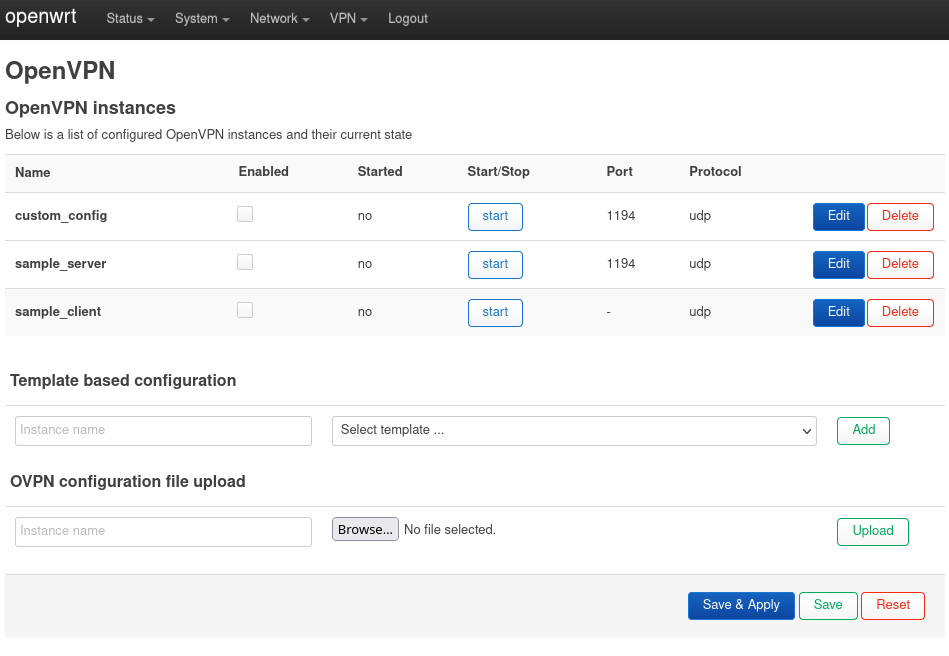
\includegraphics[width=0.9\textwidth]{immagini/LuCI_vpn1}
    \caption{Configurazione della VPN tramite LuCI}
    \label{fig:luci-vpn}
\end{figure}

alla riga "custom\_config" Si deve mettere il check su \it{enabled} e premere start, per poi salvare le modifiche. In questo modo il router si connetterà automaticamente alla VPN anche se venisse riavviato.


% <-- section -->
\section{Abilitazione del Client-to-Client nel server OpenVPN}

In questo momento i client della VPN, \it{client1} e \it{router}, possono comunicare tra loro, ma lo fanno passando per la network stack del \it{server}. Infatti:

\begin{bashcode}{Router 4g}{}
$ ping -c2 10.8.0.2                  # client1
PING 10.8.0.2 (10.8.0.2): 56 data bytes
64 bytes from 10.8.0.2: seq=0 ttl=63 time=0.519 ms
64 bytes from 10.8.0.2: seq=1 ttl=63 time=0.501 ms

--- 10.8.0.2 ping statistics ---
2 packets transmitted, 2 packets received, 0% packet loss
round-trip min/avg/max = 0.501/0.510/0.519 ms
\end{bashcode}

Dal server possiamo vedere i pacchetti con \it{tcpdump}:

\begin{bashcode}{Server}{}
$ sudo tcpdump -i tun0
listening on tun0, link-type RAW (Raw IP), snapshot length 262144 bytes
16:20:50.791063 IP 10.8.0.3 > 10.8.0.2: ICMP echo request, id 1759, seq 0, length 64
16:20:50.791098 IP 10.8.0.3 > 10.8.0.2: ICMP echo request, id 1759, seq 0, length 64
16:20:50.791273 IP 10.8.0.2 > 10.8.0.3: ICMP echo reply, id 1759, seq 0, length 64
16:20:50.791285 IP 10.8.0.2 > 10.8.0.3: ICMP echo reply, id 1759, seq 0, length 64
16:20:51.791153 IP 10.8.0.3 > 10.8.0.2: ICMP echo request, id 1759, seq 1, length 64
16:20:51.791174 IP 10.8.0.3 > 10.8.0.2: ICMP echo request, id 1759, seq 1, length 64
16:20:51.791365 IP 10.8.0.2 > 10.8.0.3: ICMP echo reply, id 1759, seq 1, length 64
16:20:51.791374 IP 10.8.0.2 > 10.8.0.3: ICMP echo reply, id 1759, seq 1, length 64
\end{bashcode}

Si vede che ogni richiesta viene duplicata, la prima è in entrata sulla network stack del \it{server} e la seconda in uscita. 
% TODO forse da mettere lo schema che fa vedere la network stack?
Per evitare questo traffico possiamo abilitare l'opzione \code{client-to-client} nel file di configurazione del server. In questo modo il layer openvpn effettuerà direttamente il forwarding tra i client della vpn \cite{client-to-client}.

\begin{bashcode}{Server}{}
$ vim /etc/openvpn/server/server.conf
209  client-to-client
$ sudo systemctl restart openvpn-server@server.service
\end{bashcode}

Possiamo quindi rieseguire gli stessi test fatti sopra:

\begin{bashcode}{Router 4g}{}
$ ping -c2 10.8.0.2
PING 10.8.0.2 (10.8.0.2): 56 data bytes
64 bytes from 10.8.0.2: seq=0 ttl=64 time=0.351 ms
64 bytes from 10.8.0.2: seq=1 ttl=64 time=0.307 ms

--- 10.8.0.2 ping statistics ---
2 packets transmitted, 2 packets received, 0% packet loss
round-trip min/avg/max = 0.307/0.329/0.351 ms
\end{bashcode}

Ma questa volta la network stack del \it{server} non vede nessun pacchetto:

\begin{bashcode}{Server}{}
$ sudo tcpdump -i tun0
listening on tun0, link-type RAW (Raw IP), snapshot length 262144 bytes
\end{bashcode}


\section{Assegnazione ip statico al Router}

Dato che non possiamo sapere a priori quanti client si connetteranno contemporaneamente alla VPN, per sapere sempre quale ip viene assegnato al router è necessario assegnargliene uno statico.

% TODO aggiungi per che serve la ccd
Questo viene fatto usando la \code{cleint-config-dir}.

\begin{bashcode}{Server}{}
$ sudo mkdir /etc/openvpn/server/ccd    # creo la client-config-dir
$ sudo vim /etc/openvpn/server/server.conf   # abilito l'opzione nella config del server
167  client-config-dir ccd
$ sudo vim /etc/openvpn/server/ccd/router
ifconfig-push 10.8.0.254 255.255.255.0  # impongo l'ip per questo common name
$ sudo systemctl restart openvpn-server@server.service
\end{bashcode}

Cosi' facendo al router gli verrà sempre assegnato l'ip \code{10.8.0.254}, indipendentemente dall'ordine in cui gli host si connettono alla vpn. Ciò ci permette di sapere sempre e a priori qual è l'ip del router.
